\section{Part 2}

The second part of step four builds on the skills obtained in part one,
requiring students to increase the number of memory addresses used and the size
of each stored value, while still creating an accurate reproduction of the data
after storage has been completed.

\subsection{Schematic}
Like with part one, the schematic for this expanded RAM use case was provided
in the lab instructions.  The schematic as simulated is included here in
Figure~\ref{f:schem2}.
%
\begin{figure}[H]
\centering
	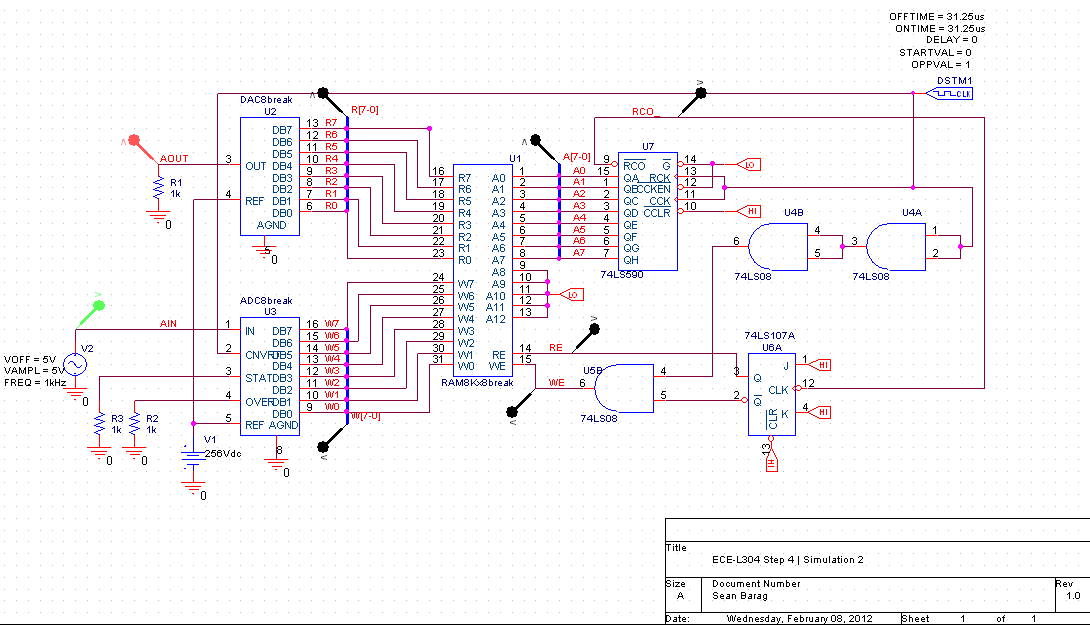
\includegraphics[width=.8\textwidth]{img/shot/schem2.png}
	\parbox{.8\textwidth}{
	\caption[Part 2 Schematic]{PSpice schematic for the circuit simulated in
	part two of step four.}
	\label{f:schem2}}
\end{figure}
%
The schematic shown reads~256 values of~8-bit data from the \ttt{W} register
(the output of an ADC) and stores them in addresses~\ttt{0x00}
through~\ttt{0xFF} in memory.  These values are subsequently read from those
locations and written to the \ttt{R} register for conversion to analog and
final output.

\subsection{Simulation}
This system has a clock period of~\SI{62.5}{\micro\second}, corresponding to a
clock frequency of~\SI{16}{\kilo\hertz}.  Since there are~256 addresses being
utilized~(each for both read and write), the simulation lasted
for
%
\begin{equation*}
\SI{256}{Addresses} \cdot \SI{2}{Accesses\per Address} \cdot
	\SI{62.5}{\micro\second\per Access} = \SI{32}{\milli\second} \quad \text{.}
\end{equation*}

Initially, the ADC and DAC were driven by a~\SI{256}{\volt} source.  The
resulting output, as calculated by PSpice, is shown in
Figure~\ref{f:schem2plot1}.
%
\begin{figure}[H]
\centering
	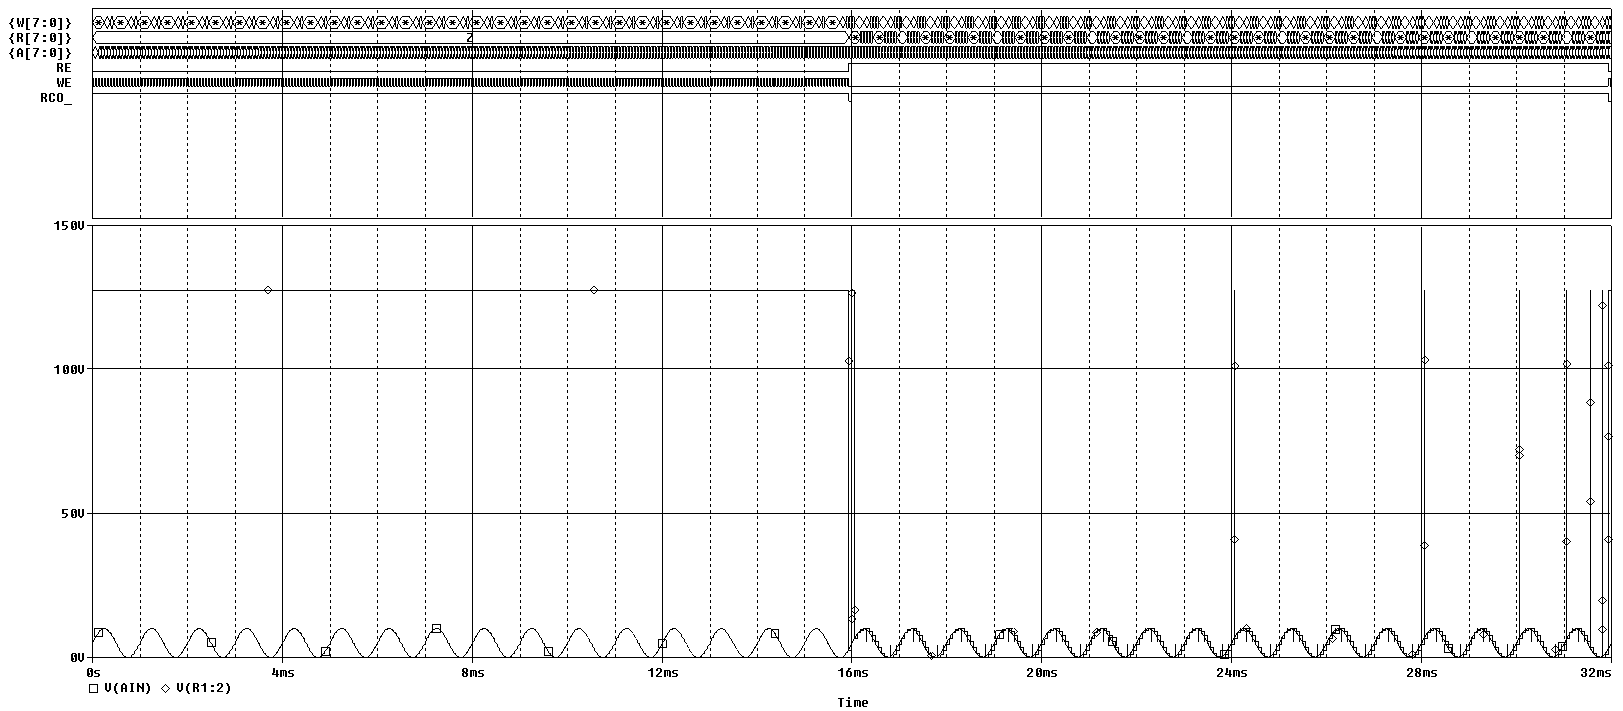
\includegraphics[width=.8\textwidth]{img/shot/sim2_plot1.png}
	\parbox{.8\textwidth}{
	\caption[Part 2 Simulation Results 1]{Results of simulating the schematic
	shown in Figure~\ref{f:schem2} for one full read-write cycle (in this
	case~\SI{32}{\milli\second}) with a~\SI{256}{\volt} supply.  A larger
	version of this figure is available in appendix
	Figure~\ref{f:schem2plot1_big}.}
	\label{f:schem2plot1}}
\end{figure}
%
While the output appears to represent the input fairly accurately, the output
is clamped at roughly~\SI{125}{\volt} while the system is reading data.
Additionally, there are occasional spikes in output voltage to the
same~\SI{125}{\volt} level that seem to correspond to addresses with only
consecutive ones in the most significant bits~(e.g. \ttt{1000 0000}, \ttt{1100
0000}, \ttt{1110, 000}, \ldots).  This phenomenon was prevented by changing the
ADC and DAC supplies to just~\SI{10}{\volt}, which produced the plot shown in
Figure~\ref{f:schem2plot2}.
%
\begin{figure}[H]
\centering
	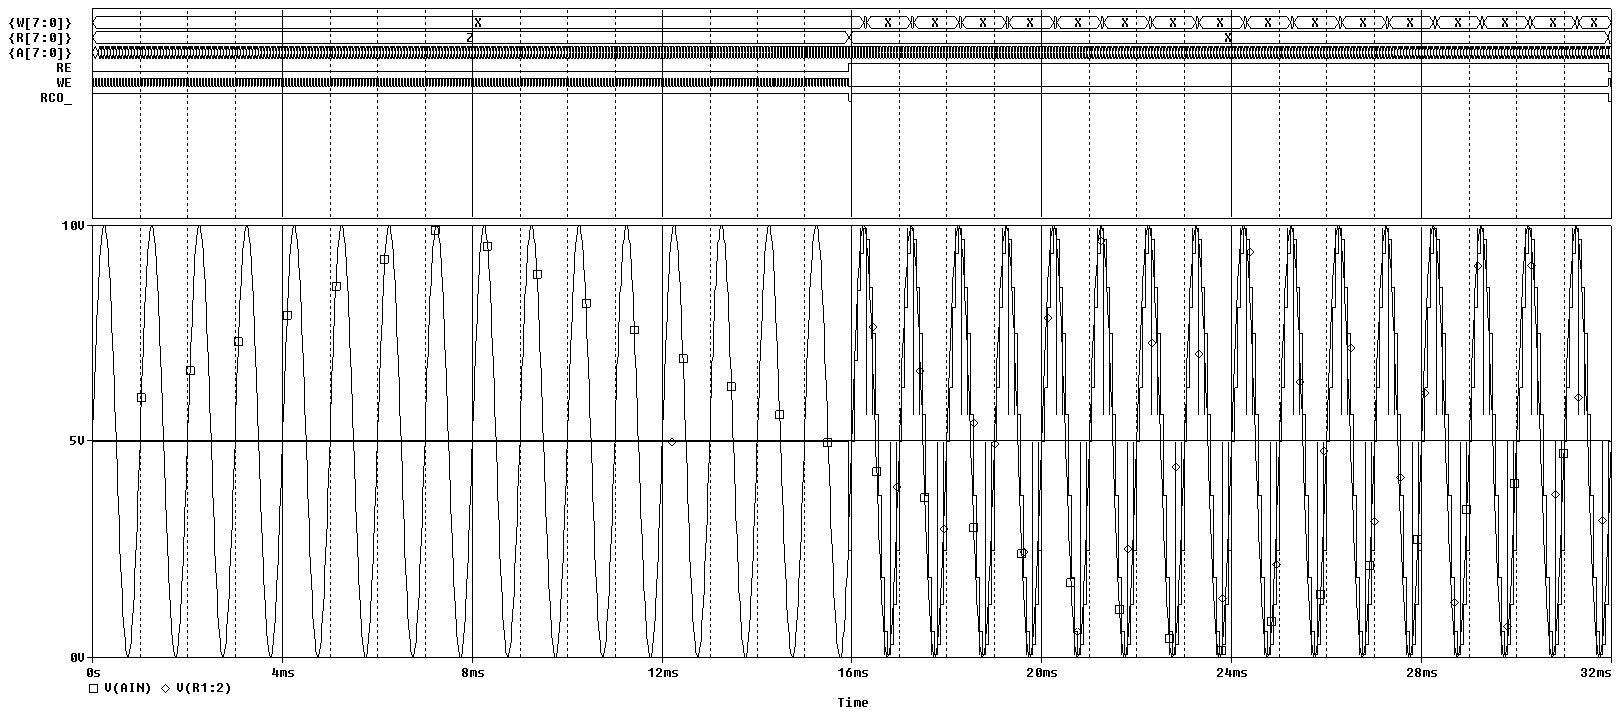
\includegraphics[width=.8\textwidth]{img/shot/sim2_plot2.png}
	\parbox{.8\textwidth}{
	\caption[Part 2 Simulation Results 2]{Results of simulating the schematic
	shown in Figure~\ref{f:schem2} for one full read-write cycle (in this
	case~\SI{32}{\milli\second}) for a supply voltage of~\SI{10}{\volt}.  A
	larger version of this figure is available in appendix
	Figure~\ref{f:schem2plot2_big}.}
	\label{f:schem2plot2}}
\end{figure}
%
After making this modification to the supply voltage, the output still clamps
to half the supply voltage while reading data.  Since this is
just~\SI{5}{\volt} now, there is no risk of damaging components.  While spikes
to half-supply voltage are still present, they are now periodic, and appear to
occur twice per period of sinusoidal input.  Regardless, the input and output
waveforms match well within the limitations of the~8 bit ADC and DAC
resolutions.  As this system is merely an extension of the one in part one, the
relationships between the \ttt{A}, \ttt{W}, \ttt{R}, and \ttt{RW} registers
remains the same, and the proper read/write timing rules are still followed.

After careful observation, it can be seen that there is a propagation delay for
values to pass through the L4S590 counter IC equal to the period of one full
clock cycle.  This is evident by the time between~$t = 0$ and the first
non-zero value plotted in Figures~\ref{f:schem2plot2}
and~\ref{f:schem2plot2_big}.  Similarly, there is a lag between when \ttt{RE}
goes high and when the first valid data is produced.  This is equal to two full
clock periods~(\SI{62.5}{\micro\second}); one for the counter to reset, and
another for the reset to propagate through the device.

